\subsection{Übergangsamplituden}
Betrachte eindimensionale Probleme

Mechanik:
	\begin{align*}
		L(x,\dot{x}) &= 
		\frac{m}{2} \dot{x}^2 - V(x),&
		\text{kanonischer Impuls } p&= \frac{\partial L}{\partial \dot{x}}\\
		H(x,p) &= \dot{x}p(x,\dot{x}) - L(x, \dot{x}) = \frac{p^2}{2m} - V(x)
	\end{align*}
	\begin{align*}
		H\ket{n} &= E_n \ket{n} ,& 
		\braket{n | m} &= \delta_{mn} ,& 
		\sum_n \ket{n} \bra{n} &= \mathds{1} \\
		\text{Ortsoperator} \\
		\hat{x} \ket{x} &= x \ket{x} ,&
		\braket{x | x'} &= \delta(x - x') ,&
		\int \diff x \ket{x} \bra{x} &= \mathds{1} \\
		\text{Beliebiger Zustand }
		&\ket{\psi} ,&
		\psi(x) &= \braket{x | \psi} ,&
		\text{insbesondere } \braket{x | n} &= \psi_n(x)
	\end{align*}
Schrödingergleichung
	\begin{align*}
		H \ket{\psi(t)} &= i \hbar \frac{\partial}{\partial t} \ket{\psi(t)}
		& &\Rightarrow \psi(t) = \U_t \ket{\psi(0)} \\
		\text{mit } \U_t &= e^{-\frac{i}{\hbar} H t} & &\text{Unitärer Zeitentwicklungsoperater}
	\end{align*}
(Zeitordung wäre notwenig, falls $V(x,t) t$-abhängig wäre)
	\begin{align*}
		\Rightarrow \ket{x(t)} &= \U_t \ket{x(0)} = \U_t \ket{x} 
	\end{align*}
Übergangselement von Position $x_i$ zur Zeit $t_i$ nach $x_f$ zur Zeit $t_f$ 
	\begin{align*}
		|\braket{x_f | x_i}|^2 :& \text{ Wahrscheinlichkeitsdichte von, wenn ich bei }x_i\text{ starte,}\\ &\text{ komme ich bei }x_f\text{ an} \\
		_H\braket{x_f;t_f | x_i; t_i}_H &=
		\braket{x_f(t_f) | \U_{t_f} \U_{t_i}^\dagger | x_i(t_i)} \\
		&= \braket{x_f(t_f) | \exp \left(-\frac{i}{\hbar} H(t_f-t_i)\right) | x_i(t_i)}\\
		&= \sum_n \braket{x_f | n} \braket{n | x_i} e^{-\frac{i}{\hbar} E_n (t_f - t_i)} \\
		&= \sum_n \psi_n (x_f) \psi^*_n(x_i) e^{-\frac{i}{\hbar} E_n (t_f - t_i)}
	\end{align*}
Übergangsamplitude enthält Information ber Wellenfunktionen $\psi_n(x)$ und Energien $E_n$ 
\\
Alternative Formulierung der Quantenmechanik:

``Pfadintegrale'' erlauben Berechnung von Korrelationsfunktionen (Dirac 1931, Feynman 194..), z.B. $_H\braket{x_f | \hat{x} (t_2) \hat{x} (t_1) | x_i}_H$, ohne dass die Schrödingergleichung gelöst werden muss. 
\\
Diskretisiere die Zeit:
	\begin{align*}
		\ket{x_j}_H &= \ket{x_j ; t_j}_H ,&
		t_j &= j \cdot a ,& t_i &= t_0 = t = 0,&
		t_f &= t_N = Na \\
		\text{mit } a &= \frac{t_f}{N} ,& N &\in \mathds{N}
	\end{align*}
	\begin{figure*} [h]
		\begin{center}
			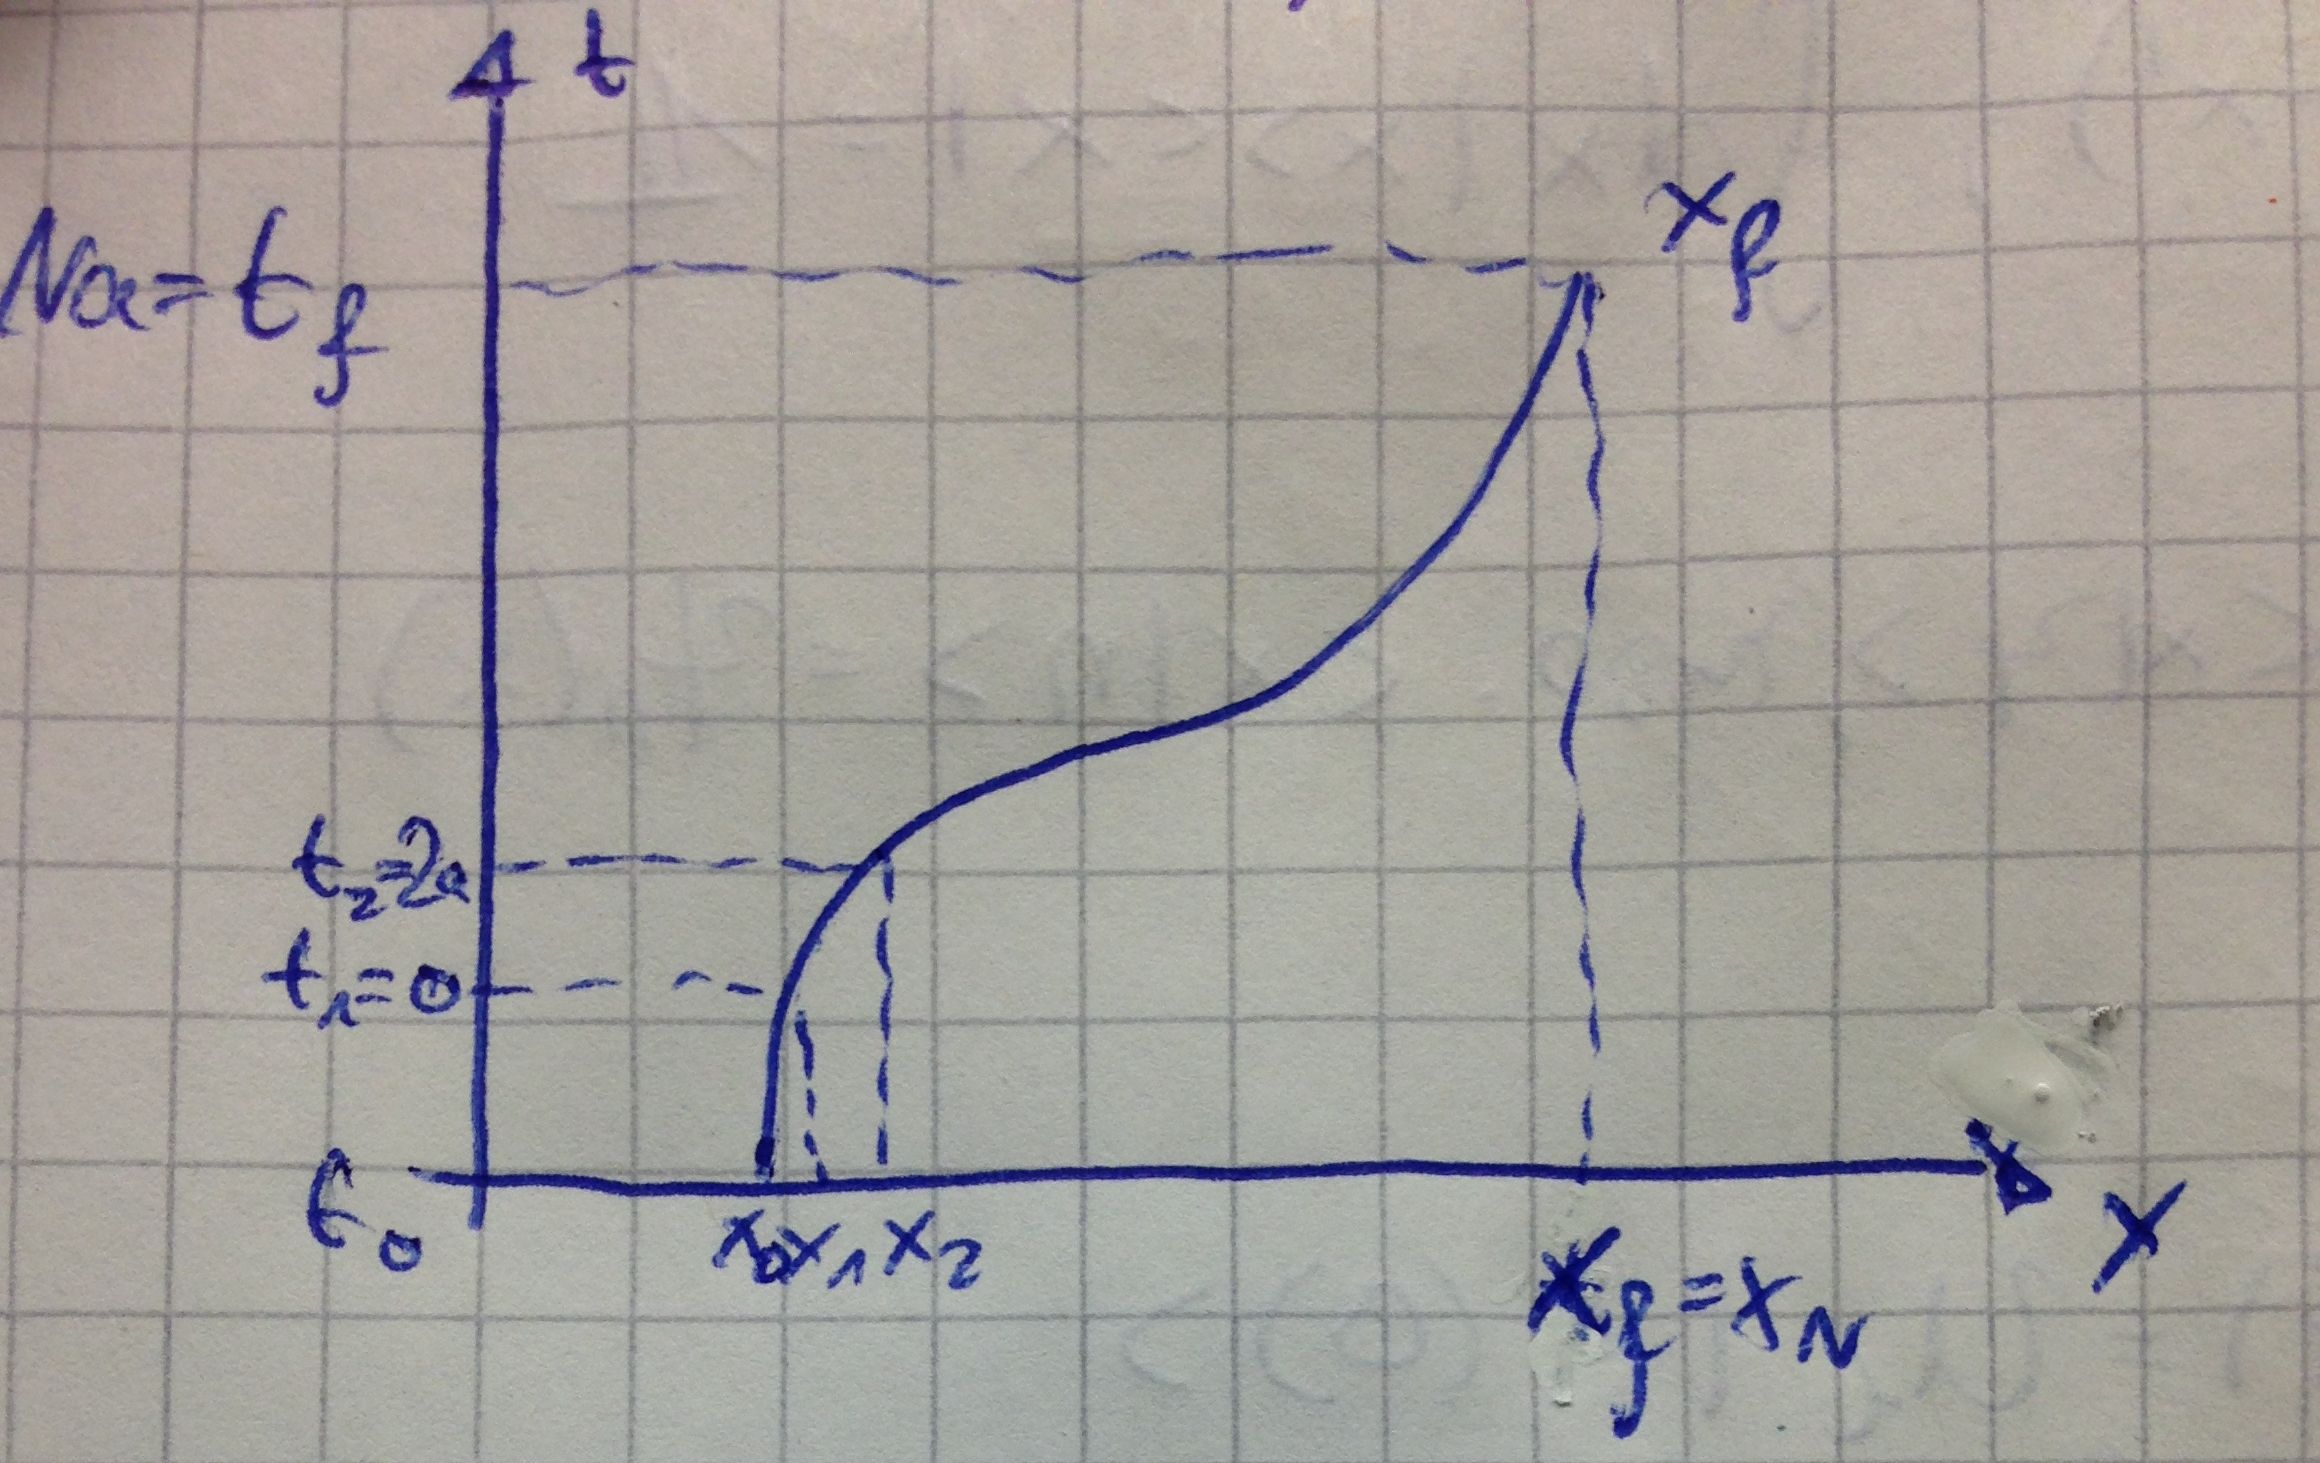
\includegraphics[width=10cm]{Uebergangsamplituden1}
		\end{center}
	\end{figure*}
Setze ein: $\mathds{1} = \int \diff x_j \ket{x_j}_H \vphantom{\bra{x_j}}_H\bra{x_j}$
	\begin{align*}
		&\Rightarrow _H\braket{x_f | x_i}_H^{(N)} 
		\left(\underset{N\rightarrow \infty , a \rightarrow 0}{\longrightarrow} \vphantom{\braket{x_f | x_i}}_H\braket{x_f | x_i}_H\right) \\
		&= \int \vphantom{\braket{x_f | x_i}}_H\braket{x_f | x_{N - 1}}_H \diff x_{N-1} \vphantom{\braket{x_f | x_i}}_H\braket{x_{N-1} | x_{N-2}}_H 
		\diff x_{N-2} \vphantom{\braket{x_f | x_i}}_H\braket{x_{N-2} | \ldots | x_1}_H
		\diff x_1 \vphantom{\braket{x_f | x_i}}_H\braket{x_1 | x_i}_H
	\end{align*} 
Was ist $_H\braket{x_{j+1} | x_j}_H$?

Transferoperator:
	\begin{align*}
		\hat{\mathrm{T}} &= e^{-\frac{i}{\hbar} H a} ,&
		\hat{\mathrm{T}}^N &\approx \U_t
	\end{align*}
	\begin{align*}
		_H\braket{x_{j+1} | x_j}_H &= {}_H\braket{x_{j+1}| \hat{\mathrm{T}} | x_j}_H \\
		&= {}_H \braket{x_{j+1} | e^{-\frac{ia}{\hbar} \left(\frac{\hat{p}^2}{2m} + V(x)\right)} | x_j}_H \\
		&= {}_H \braket{x_{j+1} | e^{-\frac{ia}{2\hbar} V(x_{j+1})} e^{-\frac{ia}{2\hbar}V(x_j)} | x_j}_H (1 + \mathscr{O}(a^2))
	\end{align*}
	\begin{align*}
		_H\braket{x_{j+1} | x_j}_H &=
		{}_H\braket{x_{j+1} | e^{-\frac{ia}{\hbar} \frac{\hat{p}^2}{2m}} | x_j}_H
		e^{-\frac{ia}{\hbar} \left(V(x_j) + V(x_{j + 1})\right)}
	\end{align*}
Füge ein:
	\begin{align*}
		\int \frac{\diff p}{2 \pi} \ket{p} \bra{p} &= \mathds{1} ,& 
		\braket{x | p} &= e^{\frac{i}{\hbar} xp}
	\end{align*}
	\begin{align*}
		_H\braket{x_{j+1} | e^{-\frac{ia}{\hbar} \frac{\hat{p}^2}{2m}}| x_j}_H
		&= \int \frac{\diff p}{2 \pi} e^{\frac{i}{\hbar} (x_{j+1} - x_j)}  e^{-\frac{ia}{\hbar} \frac{\hat{p}^2}{2m}} \\
		&= \sqrt{\frac{m}{2 \pi i a}} \exp\left(\frac{im}{2 \hbar a} (x_{j+1} - x_j)\right)^2 \\
		&= \sqrt{\frac{m}{2 \pi i a}} \exp\left[\frac{ia}{\hbar} \frac{p_j^2}{2m}\right]
		(1 + \mathscr{O}(a^2)) \\
		_H\braket{x_{j+1} | x_j}_H &=
		\sqrt{\frac{m}{2 \pi i a}} e^{\frac{ia}{\hbar} \left[\frac{p_j^2}{2m} - \frac{1}{2} V(x_{j+1}) - \frac{1}{2} V(x_i)\right]} \\
		&\propto \exp (i \frac{a}{\hbar} L_j)
	\end{align*}
\underline{Pfadintegrale} (1.dim) \marginpar{10.12.15}
\marginpar{nicht von Prof.Bali gehalten}
	\begin{figure*} [h]
		\begin{center}
			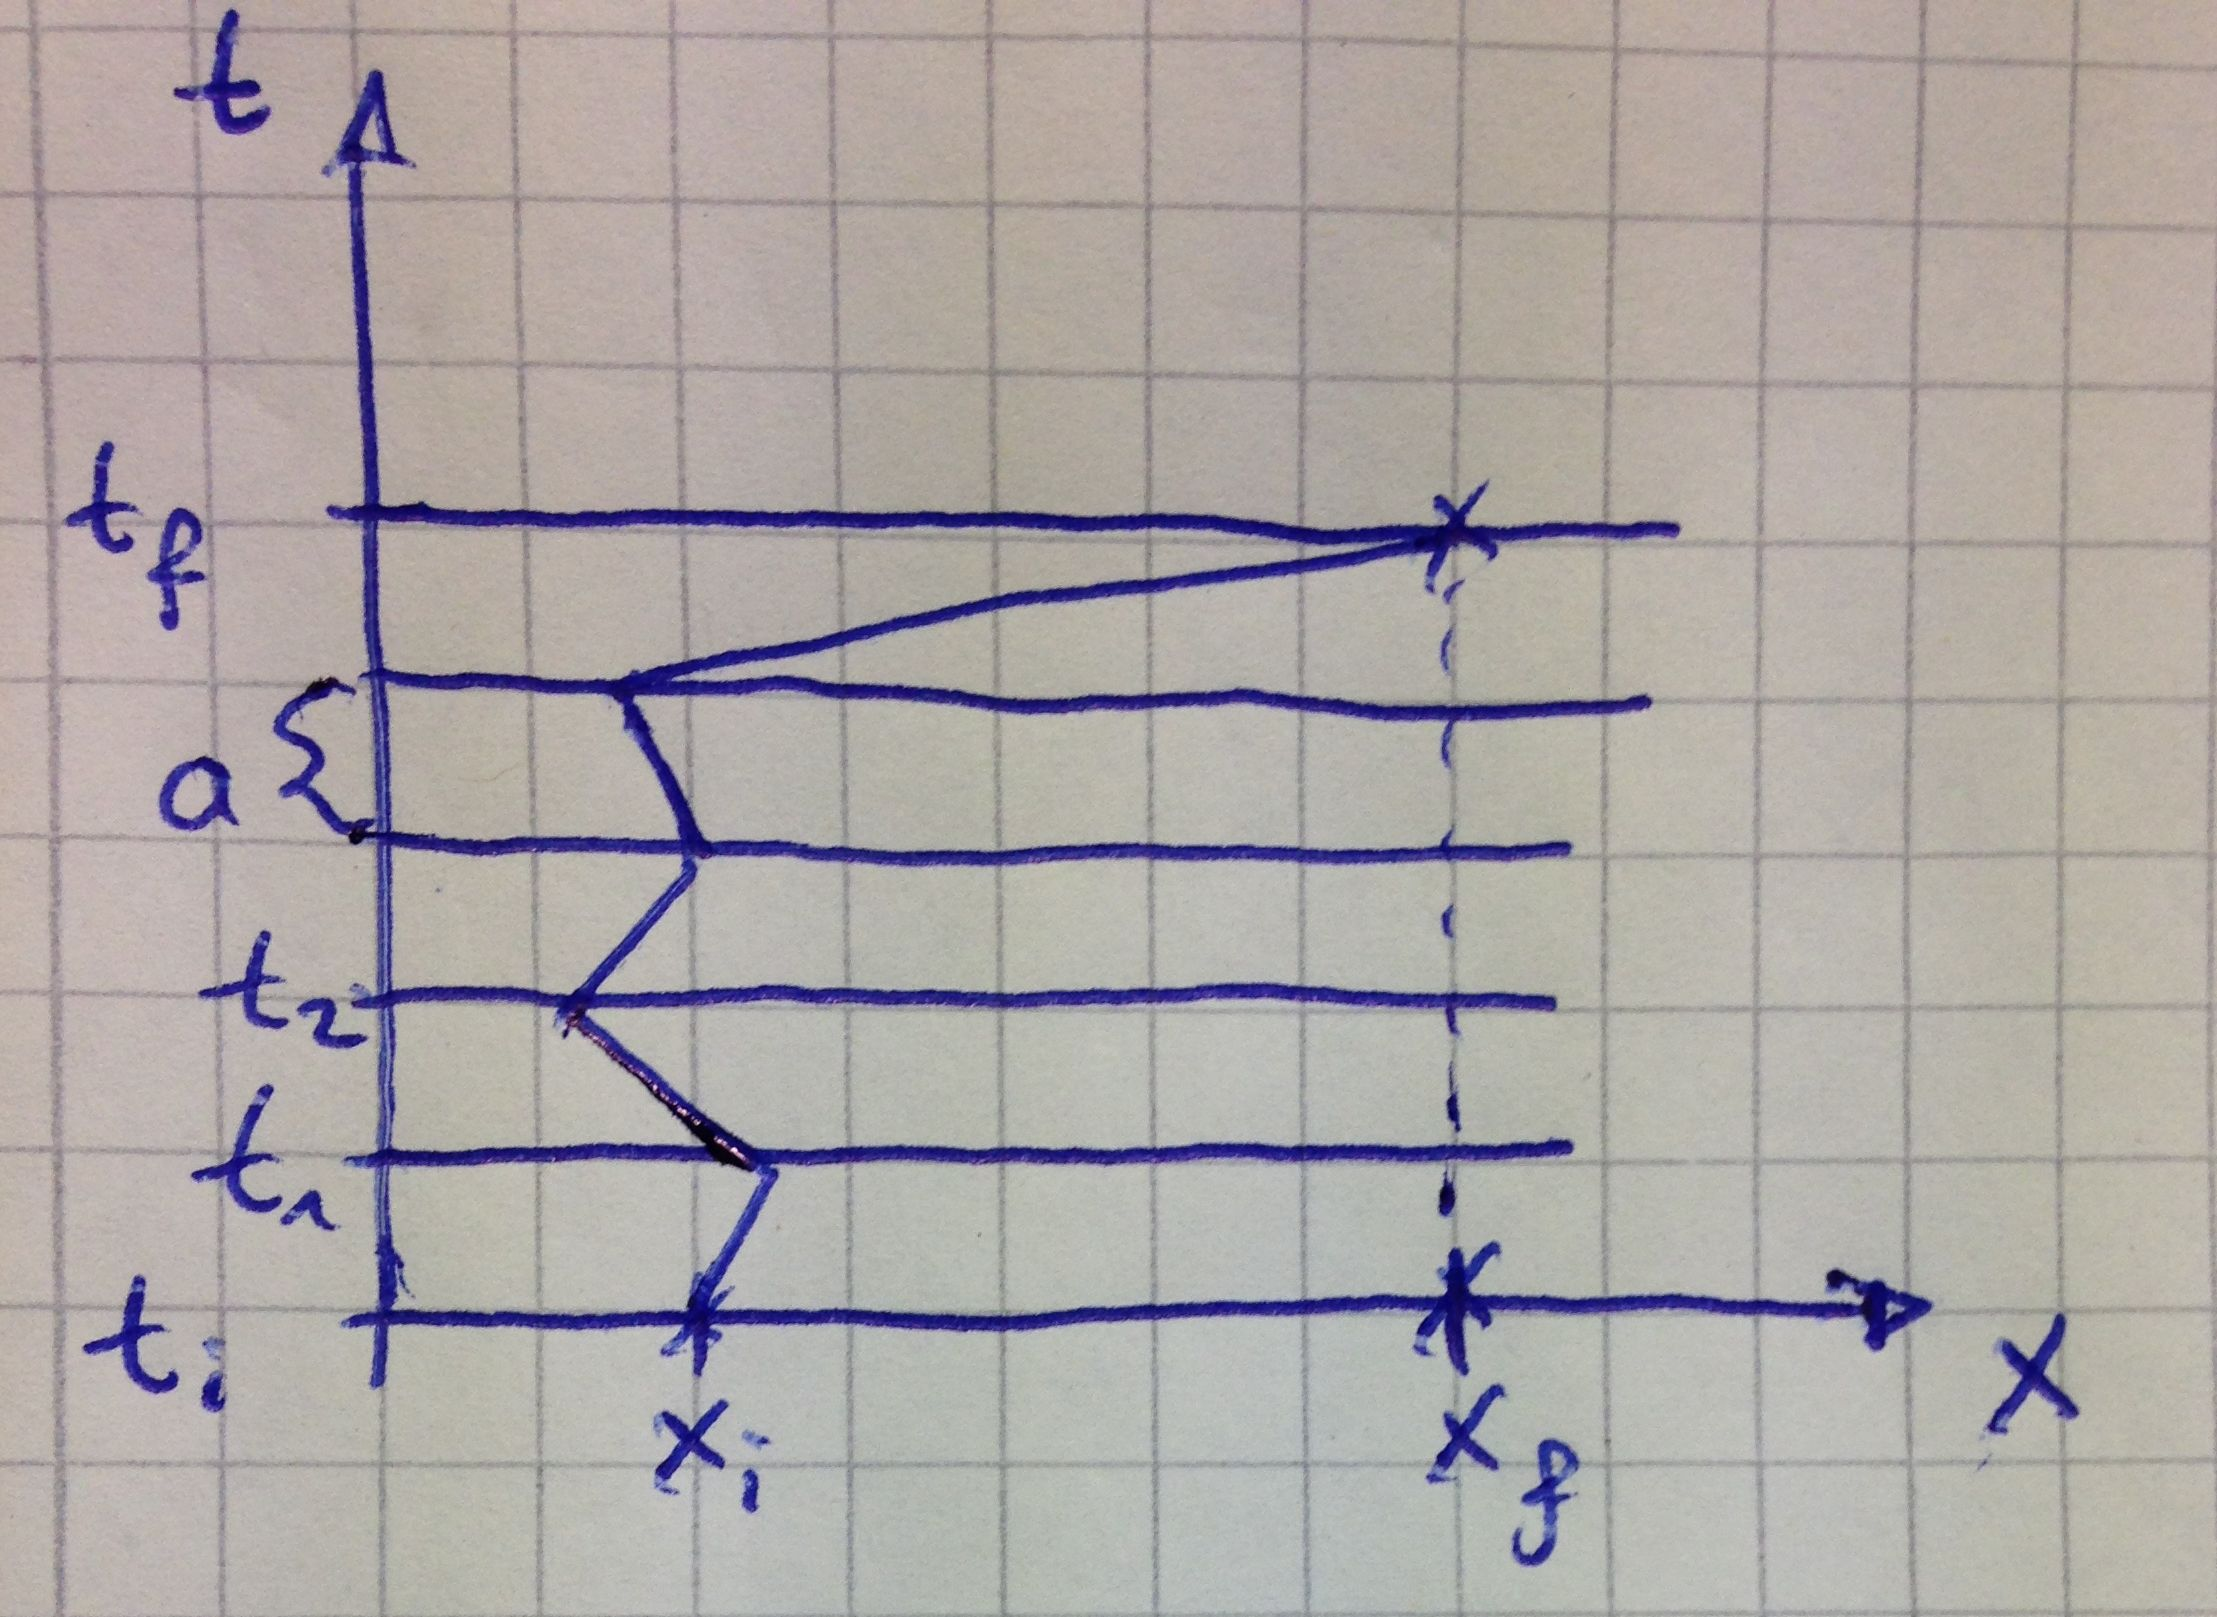
\includegraphics[width=10cm]{Uebergangsamplituden2}
		\end{center}
	\end{figure*}